\chapter{Métodos Supervisados}

%Supongamos que tenemos un conjunto de variables, $\textbf{X}$ que influyen sobre una o más variables conocidas $\textbf{Y}$. A partir de ahora, las llamaremos variables de entrada y variables objetivo respectivamente. El principal propósito de los métodos supervisados, es dado una muestra de individuos con observaciones de ambos tipos de variables predecir la variable objetivo para nuevos individuos de los que solo conozcamos las variables de entrada  
%
%Para empezar tenemos que fundamentar de manera teórica como calcular esa función para predecir. 
%\section{Teoría de decisión estadística}
Sea $X\in \mathbb{R}^p$ un vector aleatorio real e $Y \in \mathbb{R}$ una variable aleatoria real. En este contexto, $X$ e $Y$ serán las variables de entrada y la variable de salida respectivamente. Asimismo, sea $\mathbb{P}(X,Y)$ la distribución de probabilidad conjunta.   

Se busca una función $f(X)$ para predecir $Y$. Dicho predictor tiene asociada una pérdida, es decir, una forma de penalizar el error de predicción. En esta memoria, a no ser que se explicite utilizaremos el error cuadrático para las regresiones, $L(Y,f(X))=(Y-f(X))^2$ . 

\begin{defi}
Llamaremos error de predicción esperado de $f$ o $EPE(f)$ a la siguiente expresión:
\begin{equation}
EPE(f)=E(Y-f(X)^2)=\int (y-f(x))^2 \mathbb{P}(dx,dy)
\end{equation}

\noindent A priori se conocen los valores de $X$, entonces si condicionamos a dichos valores, obtenemos que $\mathbb{P}(Y,X)=\mathbb{P}(Y|X)\cdot\mathbb{P}(X)$ aplicándolo en la expresión anterior resulta que 
\begin{equation}
\begin{split}
EPE(f)&=\int (y-f(x))^2 \mathbb{P}(dx,dy)=\int\int (y-f(x))^2 \mathbb{P}(dy|dx)\mathbb{P}(dx)\\
&= \mathbb{E}_X(\mathbb{E}_{Y|X}((Y-f(X))^2|X))
\end{split}
\end{equation}

\end{defi}

\noindent Este parámetro nos ofrece un criterio para encontrar $f$, es decir, $f$ será la que minimice el $EPE(f)$ , en concreto, $f(x)=\mathbb{E}(Y|X=x)$. Añadir que este sería el caso de la regresión. 

\noindent No obstante, para los casos de \textbf{clasificación} cambia el hecho de que la función cuadrática de pérdida no es adecuada. Sea $G$ una variable categórica con $K$ distintos valores posibles, entonces su función de pérdida se puede expresar como una matriz \textbf{L}. Podemos definir el termino $l_{i,j}=$``Pérdida de clasificar como $G_i$ lo que en realidad es  $G_j$". Lo más frecuente es tomar la pérdida $0-1$, esta asigna 0 a las muestras correctamente clasificadas y 1 a las no categorizadas de manera satisfactoria. 

\noindent Con esta función de pérdida el error de predicción esperado pasa a ser: 

%\input{Documentos Extra/Regresion Lineal Multiple.tex}
%\input{Documentos Extra/Clasificacion Lineal Multiple.tex}

\noindent Sea un conjunto de variables aleatorias observables de manera simultánea en una población. Estas variables se pueden dividir en dos tipos \cite{Hastie 2001}:
\begin{itemize}
\item \textbf{\textit{Variables de entrada o predictoras}}: Son las variables independientes que determinarán de manera aleatoria al segundo conjunto de variables. Al conjunto de variables aleatorias de entrada se la denotará como el vector aleatorio $\textbf{x}=[X_1,\ldots X_p]$. \\
\begin{defi}
Tomando $N$ observaciones de estas variables  de manera simultánea se obtiene la \textit{matriz de datos} $\textbf{X}$. Esta matriz es de tamaño $N\times p$ y contiene como filas los vectores de longitud $p$ que representan los datos de cada observación, se denotarán a lo largo de la memoria como $\textbf{x}_i, i=1\ldots N$. Por ejemplo, en el caso de que se recojan datos sobre distintos modelos de coches las observaciones serían los valores medidas de las distintas variables consideradas en cada uno de los coches. 
\end{defi}
\item \textbf{\textit{Variables de salida }}: Son las variables dependientes de las anteriores. A este conjunto de variables se les denota con el vector aleatorio $\textbf{y}=[Y_1,\ldots Y_K]$, en el caso de que se tenga una única variable respuesta se denotará como $Y$. \\
Como en el caso de las variables de entrada, se tomarán $N$ observaciones de las $K$ variables, dando como resultado la matriz de respuestas $\textbf{Y}$ de tamaño $N \times K$, donde cada observación es una fila y se denota como $\mathbf{y}_i, i=1\ldots K$, en el caso de que $K>1$ y como $y_i$ cuando $K=1$. Siguiendo el ejemplo anterior, se podrían tener variables respuesta como el tipo de etiqueta medioambiental siendo esta una variable discreta o el precio del vehículo que tiene naturaleza continua. 
\end{itemize}
\noindent Por ende, se recogen observaciones simultáneas de las variables de entrada y de salida formando parejas $(\mathbf{y}_i,\textbf{x}_i), i=1\ldots N$, de manera que se obtiene un vector fila de tamaño $p+K$. Estas observaciones de las variables forman una muestra aleatoria de la población .
\begin{defi}
Se llama \emph{muestra aleatoria} de una variable aleatoria con una cierta distribución de probabilidad $F$, a un conjunto de $N$ variables aleatorias con la misma distribución. 
\end{defi} 

\begin{defi}
Se llaman métodos supervisados \cite{Mahesh 2020} a aquellos métodos que buscan inferir una relación estocástica entre dos grupos de variables, predictoras y respuesta en un conjunto de datos contiene observaciones simultaneas de ambos conjuntos de datos. 
\end{defi}

\noindent Durante la memoria, se establecerán los fundamentos a nivel poblacional, solo teniendo en cuenta las propiedades de las variables aleatorias y luego en caso de que sea necesario se tomarán $N$ observaciones o realizaciones del experimento para formar las matrices de datos correspondientes. 

\noindent En conclusión, el objetivo de estos métodos supervisados es encontrar una relación estocástica que llamaremos predictor, de tal manera que para una nueva observación de las variables de entrada, que denotaremos con $\textbf{x}_0$, se pueda hacer una predicción $\hat{\textbf{y}}_0$ del valor real $\textbf{y}_0$ de la variable respuesta siempre con un cierto error que será una variable  aleatoria. 
 

\input{Documentos Extra/MétodosLinealesRegresion.tex}
\newpage
\section{Métodos de Clasificación y Discriminación}

\noindent Los métodos de clasificación buscan separar los elementos de un espacio de observaciones en grupos conocidos previamente. 

\begin{defi}
Llamaremos \textit{discriminación o análisis discriminante} a aquel que busca describir las características principales de cada uno de los grupos o clases mediante \textit{funciones discriminantes} 
\end{defi}

\begin{defi}
Llamaremos \textit{métodos de clasificación} a aquellos que dada una nueva observación, \textbf{x}, buscan predecir con la máxima precisión a que clase pertenecen mediante \textit{reglas de clasificación}
\end{defi}

\noindent Hay que señalar que no siempre hay una diferencia clara entre ambas disciplinas y que puede haber veces que ambas se solapen. 


\subsection{Análisis Discriminante}

\noindent Según \textit{Lebart L., Morineau, A. y Warwick K.M.} \cite{Lebart 1984} el análisis discriminante es un conjunto de técnicas que permiten describir y clasificar un gran número de observaciones de las cuales se han medido una gran cantidad de variables. 

\noindent El método que se describe aquí es un método supervisado ya que se conocen las clases a las que pertenecen cada una de las observaciones. 



\subsection{Formalización del Análisis Discriminante}
 
\noindent Sea \textbf{X} la matriz de datos de tamaño $n \times p$
donde las filas $\textbf{x}_i$ son cada una de las observaciones de las $p$ variables. Dichas observaciones están particionadas en general por $q$ grupos, sea $I_k$ el conjunto de observaciones pertenecientes al $k$-ésimo grupo, sea también $n_k$ el número de observaciones que pertenecen al $k$-ésimo grupo.

\noindent Se definen las medias muestrales $\overline{x}_j=\frac{1}{n}\sum_{i=1}^n x_{ij}$ de la $j$-ésima variable en la población en total. También se define la media muestral dentro de cada grupo que es $\overline{x}_{jk}=\frac{1}{n_k}\sum 
_{i\in I_k} x_{ij}$ 

\noindent Por ende podemos dar la distancia entre dos variables como:
\begin{align}
Cov(X_j,X_{j'})&=\dfrac{1}{n}\sum_{i=1}^n(x_{ij}-\overline{x}_j)(x_{ij'}-\overline{x}_j')
\intertext{Esto se puede particionar por grupos de la siguiente manera: }
Cov(X_j,X_{j'})&=\dfrac{1}{n}\sum_{k=1}^q\sum_{i\in I_k}(x_{ij}-\overline{x}_j)(x_{ij'}-\overline{x}_j')
\intertext{y a su vez cada uno de los $(x_{ij}-\overline{x}_j)$ se pueden dividir en la parte intergrupos e intragrupos: }
(x_{ij}-\overline{x}_j)&=(x_{ij}-\overline{x}_{jk})+(\overline{x}_{jk}-\overline{x}_{j})
\end{align}
Sustituyendo y simplificando lo necesario: 
\begin{equation}
Cov(X_j,X_{j'})=\dfrac{1}{n}\sum_{k=1}^q\sum_{i\in I_k}(x_{ij}-\overline{x}_{jk})(x_{ij'}-\overline{x}_{j'k})+\sum_{k=1}^q\dfrac{n_k}{n}(\overline{x}_{jk}-\overline{x}_{j})(\overline{x}_{j'k}-\overline{x}_{j'})
\end{equation}

\noindent Esto nos permite dar una descomposición de la matriz de covarianzas total de la siguiente forma :
\begin{equation}\label{descomposicion varianza}
\textbf{T}=\textbf{B}+\textbf{W}
\end{equation}

Donde:
\begin{itemize}
\item \textbf{T} es la matriz que expresa la covarianza total y sus coeficientes  $t_{jj'}=Cov(X_j,X_j')$
\item \textbf{B} es la matriz que expresa la covarianza entre los grupos y sus coeficientes son $b_{jj'}=\sum_{k=1}^q\dfrac{n_k}{n}(\overline{x}_{jk}-\overline{x}_{j})(\overline{x}_{j'k}-\overline{x}_{j'})$
\item \textbf{W} es la matriz que expresa la covarianza dentro de los grupos y sus coeficientes son $w_{jj'}=\dfrac{1}{n}\sum_{k=1}^q\sum_{i\in I_k}(x_{ij}-\overline{x}_{jk})(x_{ij'}-\overline{x}_{j'k})$
\end{itemize}

\noindent Para cualquier combinación lineal que se quiera hacer de las variables de entrada de la forma $\textbf{a}^T \textbf{x}$, donde el vector $\textbf{a}$ es un vector de $p$ constantes,  entonces la varianza se transforma de la siguiente manera:
\begin{equation}
Var(\textbf{a}^T \textbf{x})=\textbf{a}^T \Sigma \textbf{a}
\end{equation}

\noindent Entonces transformando por el vector $\textbf{a}$ tenemos que la Ecuación \eqref{descomposicion varianza} se transforma de la siguiente manera: 
\begin{equation}
\textbf{a}^T \textbf{T}\textbf{a}= \textbf{a}^T \textbf{B}\textbf{a}+\textbf{a}^T \textbf{W}\textbf{a}
\end{equation}

\noindent Recopilando, el objetivo del análisis discriminante lineal es encontrar combinaciones lineales que maximicen la varianza entre grupos y minimicen la varianza dentro de los grupos. Eso es equivalente a encontrar el vector $\textbf{a}$ tal que:
\begin{equation}
f(\textbf{a})=\dfrac{\textbf{a}^T \textbf{B}\textbf{a}}{\textbf{a}^T \textbf{T}\textbf{a}}
\end{equation}
\noindent Es máxima. Si además utilizamos la restricción $\textbf{a}^T \textbf{T}\textbf{a} = 1$. En principio la función objetiva es homogénea, es decir, $f(\mu \textbf{a})=f(\textbf{a})$
Utilizando el método de los multiplicadores de Lagrange derivamos respecto del vector $\textbf{a}$ tendremos que:
\begin{align}
L(\textbf{a})&= \textbf{a}^T \textbf{B}\textbf{a}-\lambda(\textbf{a}^T \textbf{T}\textbf{a}-1) 
\intertext{al derivarla respecto de \textbf{a} se obtiene que: }
\dfrac{\partial L(\textbf{a})}{\partial \textbf{a} } &= 2\textbf{B}\textbf{a}-2\lambda\textbf{T}\textbf{a}
\intertext{En consecuencia: }
\textbf{B}\textbf{a} &= \lambda \textbf{T} \textbf{a}
\intertext{Si además \textbf{T} es no singular}
\textbf{T}^{-1}\textbf{B}\textbf{a}&=\lambda \textbf{a}
\end{align}

Es decir, el vector $\textbf{a}$ es el vector de valor propio $\lambda$, tomando el valor propio máximo de la matriz $\textbf{T}^{-1}\textbf{B}$.

\begin{defi}
Al valor $\lambda$ se le conoce como \textit{potencia discriminante} de la combinación \textbf{a}.
\end{defi}

\begin{propo}
El desarrollo antes detallado es análogo para $f(\textbf{a})=\dfrac{\textbf{a}^T \textbf{B}\textbf{a}}{\textbf{a}^T \textbf{W}\textbf{a}}$
\end{propo}
\noindent Esto se puede ver detallado en \emph{Peña, D.} \cite{Peña 2002}. De tal manera que $\textbf{a}$

\noindent \textit{Observación} Esta técnica se diferencia del Análisis de Componentes Principales en que en el Análisis Discriminante se maximiza la distancia o variación entre grupos conocidos, mientras que el Análisis de Componentes Principales únicamente busca las direcciones en las que los datos varían más. 

\noindent Pero, en caso de ser aplicada, el análisis discriminante desarrollado aquí se puede utilizar como método de reducción de la dimensionalidad para el caso de la clasificación. De esta manera, utilizando mecanismos similares a los que se describirán en la parte del Análisis de Componentes Principales la matriz de datos puede ser reducida. 

\subsection{Métodos de Clasificación}

\noindent En la introducción de este capítulo se detalló que el clasificador Bayesiano utilizaba las probabilidades conocido el valor de la observación $\textbf{x}_0$. El caso de la regresión logística intenta modelizar el cociente de las probabilidades como una función lineal. 

\noindent \textit{Hastie et.al.}\cite{Hastie 2001} detallan el caso en profundidad cuando la variable $Y$ tiene dos posibles valores.
\begin{equation}
log \dfrac{P(Y=1|\textbf{x}=\textbf{x}_0)}{P(Y=2|\textbf{x}=\textbf{x}_0)}=\beta^T \textbf{x}_0
\end{equation}

\noindent Donde $\beta$ es un vector de longitud $p+1$ y a $\textbf{x}_0$ es una observación del vector aleatorio y se le ha añadido en la primera componente el valor constante 1.

\noindent Esto sería el caso para $2$ valores posibles pero en el caso de que se tuviesen $K$ valores posibles, se definen las siguientes funciones lineales:
\begin{equation}
log \dfrac{P(Y=j|\textbf{x}=\textbf{x}_0)}{P(Y=K|\textbf{x}=\textbf{x}_0)}=\beta_j^T \textbf{x}_0 \quad j=1\ldots K-1
\end{equation}
Por tanto, el modelo queda definido por $K-1$ funciones lineales. Es decir estamos asumiendo que la probabilidad $P(Y=j|\textbf{x}=\textbf{x}_0)$ se puede expresar como una función de la siguiente manera:
\begin{equation}
P(Y=j|\textbf{x}=\textbf{x}_0)=\dfrac{e^{\beta_j^T\textbf{x}_0}}{1+\sum_{k=1}^{K-1}e^{\beta_k^T\textbf{x}_0}} \quad j=1\ldots K-1
\end{equation}

\noindent Además, $P(Y=K|\textbf{x}=\textbf{x}_0)=\dfrac{1}{1+\sum_{k=1}^{K-1}e^{\beta_k^T\textbf{x}_0}}$. 

\noindent El ajuste de estos modelos se lleva a cabo por el método de máxima verosimilitud. Donde tendríamos que \begin{equation}
l(\theta)=\sum_{i=1}^N log(p_{g_i}(x_i;\theta))
\end{equation}
\noindent En el caso de la regresión logística $p_{j}=P(Y=j|\textbf{x}=\textbf{x}_0)$ además supóngase que se tienen únicamente dos clases o dos valores para la variable $Y$ por tanto, la verosimilitud puede ser expresada de la siguiente manera
\begin{equation}
l(\beta)
\end{equation}

\newpage
\section{Redes Neuronales}

\noindent Las redes neuronales artificiales, son modelos predictivos basados en el funcionamiento de las propias neuronas del cerebro que reciben señales de entradas de las neuronas con las cuales están conectadas, las procesan y envían el resultado a las neuronas con las que estén conectadas. 

\noindent La ventaja de este tipo de algoritmos es que en esencia, son un conjunto de parámetros y funciones de activación que pueden ser ajustados para cualquier tarea y cualquier tipo de función a aproximar solo hace falta la complejidad del modelo adecuada según \emph{Hornik, K., Stinchcombe, M., y  White, H.} \cite{Hornik 1989}.  

\noindent Una neurona artificial es mucho más simple que una neurona, \emph{López R., E. Balsa-Canto y E. Oñate} \cite{Roberto 2008} definen una neurona en términos matemáticos, pero antes hay que definir los siguientes conceptos, para los cuales se han utilizado como base \cite{Grossi 2007, Neural Designer}

\noindent Sea un vector aleatorio $\mathbf{x}$ de longitud $p$, llamamos datos de entrada a los números que se introducen en la neurona que pueden ser los propios valores observados de las 
\begin{defi}
Llamaremos \emph{pesos sinápticos} $\omega$ de una neurona, al vector de $p$ constantes que regulan la importancia de cada entrada en la neurona.  A este vector de pesos sinápticos se le puede añadir un término independiente que únicamente se sumará, se le llama \emph{sesgo} y se denota como $b$.
\end{defi}

\begin{defi}
Se llama \emph{función de activación}, $f$ de una neurona artificial a la función que transforma la suma ponderada de las entradas para obtener la salida. 

\noindent Las funciones de activación más habituales son; la función \emph{identidad} \emph{(En este caso, es como si se hiciera una simple suma ponderada de los datos de entrada)}, la función \emph{sigmoide}, la \emph{tangente hiperbólica} o la función \emph{lineal regularizada} para casos de regresión, es decir, en casos en los que la variable respuesta sea continua. En caso contrario, se pueden utilizar la \emph{función softmax} o la \emph{función de regresión logística} para casos discretos, ya que devuelven valores en el intervalo $[0,1]$ y se puede asociar con la probabilidad de pertenecer a una clase u otra. 
\end{defi}
\begin{defi}
Una \emph{neurona artificial} procesa una entrada $\textbf{x}$ de acuerdo con unos \emph{pesos sinápticos} $(b,\omega)$ que luego es transformada por una función de activación $f(\mathbf{x})$.

\noindent Una  vez definidos los elementos que forman una neurona artificial estos se utilizan de manera que se utiliza la función:
\begin{equation}
\begin{split}
g:\mathbb{R}^p &\longrightarrow \mathbb{R}\\
g(\textbf{x})&\longrightarrow g(\textbf{x};b,\omega)
\end{split}
\end{equation}
\begin{equation}
g(\textbf{x})=f\left(b+\sum_{i=1}^p \omega_i x_i\right)
\end{equation}
El siguiente diagrama proporciona una forma sencilla de entender el funcionamiento de dicho modelo, incluyendo la analogía de las neuronas biológicas. 
\end{defi}
\begin{center}
%%Hay que pedirle a Carlos que lo edite por que yo la verdad que no se 
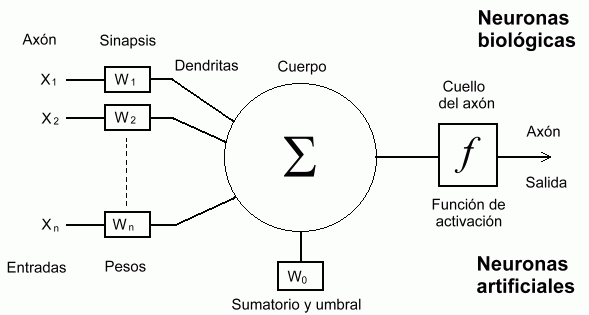
\includegraphics[scale=0.6]{Documentos Extra/Imagenes/neurona.png}
\end{center}

\noindent La principal ventaja de estos métodos es que las neuronas se pueden conectar entre ellas, es decir, estas se pueden organizar de manera que los datos de salida de un conjunto de neuronas sirvan como entrada del siguiente.
\begin{defi}
Se llama \emph{capa de neuronas} al conjunto de neuronas artificiales que tienen el mismo conjunto de datos de entrada y cuyos datos de salida para la siguiente.
\end{defi}
\noindent Se pueden establecer varios tipos de capas de neuronas \cite{Neural Designer}:
\begin{defi}
Se llama \emph{capa de entrada} a la primera capa de neuronas que recibe los valores de las observaciones y las estandariza (\emph{Se debe entrenar al modelo para ello}). Se establece una 
\end{defi}

\begin{defi}
Se llama \emph{capa oculta} a cada una de las capas intermedias que se utilizan en las redes neuronales. 
\end{defi}

\begin{defi}
Se llama \emph{capa de salida} a la última capa que tiene tantas neuronas como variables respuesta y sus datos de salida son las predicciones de 
\end{defi}

\noindent Para el proceso de ajuste se utiliza de manera habitual el método del gradiente con un conjunto de datos con $N$ observaciones. En el capitulo  11 \emph{Hastie et.al. }\cite{Hastie 2001} se detallan en profundidad el ajuste mediante el método del gradiente. De esta manera, se tiene un proceso que se llama \emph{back-propagation}. 

\noindent La siguiente imagen es una representación de una red neuornal como un grafo, en el que cada nodo es una neurona, en particular, los nodos azules son neuronas comunes, formando 5 capas ocultas, mientras que las amarillas son capas de escalado, y las rojas de salida. 

\begin{figure}[h]
\centering
%%Hay que pedirle a Carlos que lo edite por que yo la verdad que no se 
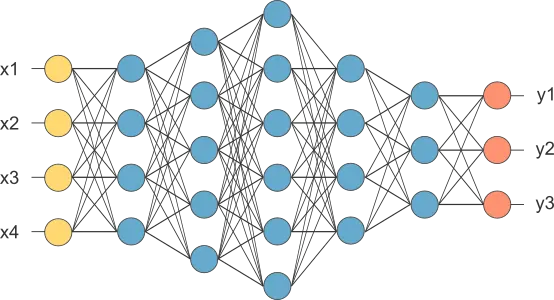
\includegraphics[scale=0.35]{Documentos Extra/Imagenes/red-neuronal-grande.png}
\caption{Imagen extraída directamente de www.neuraldesigner.com}
\end{figure}

\noindent Si se quisiera expresar el modelo como una única expresión, la expresión que se obtiene al hacer crecer un poco la red neuronal es bastante compleja de interpretar, por ejemplo en el caso anterior se tiene más de 100 parámetros y no es una red demasiado compleja, por tanto, la interpretación del modelo es compleja. Es por ello, que las redes neuronales se utilizan únicamente para fines predictivos \cite{Hastie 2001, James 2013}. 

\noindent Las principales ventajas de las redes neuronales es que pueden ajustarse a cualquier estructura sin conocerla a priori. Por otro lado, debido a la gran cantidad de parámetros a ajustar pueden provocar \emph{sobre-ajuste} pero para ello se pueden utilizar técnicas de validación cruzada \emph{(Capítulo 5 de \cite{James 2013} o el capítulo 7 de \cite{Hastie 2001})}

\noindent En esta memoria se han detallado los tipos más básicos de neuronas hay tareas específicas que este tipo de neuronas no pueden afrontar, por ejemplo, en el caso de datos que proceden de series temporales en las que estados previos influyen en los estados futuros como puede ser predicciones meteorológicas, bursátiles etc... se han desarrollado un tipo más complejo de neuronas llamadas LSTM \emph{(Long-Short Term Memory)} de las que se puede ver su desarrollo y definición además de las propiedades que poseen en \cite{Hochreiter 1997}. \emph{(Para una descripción más esquemática véase \cite{Neural Designer})}


\input{Documentos Extra/ArbolesRegresionClasificación.tex}